% 3.3.5 Desarrollo del agente conversacional (T5): estructura, interfaz interna, LLM y combinación híbrida.
% No repetir del Obj. 2: estados (fig:ob2_estados_conversacion), secuencias, contrato (tab:ob2_contrato), intenciones.
% RF14 (recordatorios) no implementado.

\subsubsection{Desarrollo del agente conversacional}

El agente se construyó en las tarjetas 11 a 13 como un servicio en Python (FastAPI) separado de la API, según la arquitectura híbrida del diseño.

\paragraph{Estructura del servicio}

El servicio sigue los puertos y adaptadores del diseño (Figura~\ref{fig:ob2_estilo_agente}): el núcleo, con la máquina de estados, no depende de WhatsApp, de la API ni del proveedor del LLM, y cada adaptador ocupa su carpeta (Figura~\ref{fig:ob3_arbol_agente}). El clasificador admite el SDK de Anthropic o una interfaz compatible con OpenAI sin cambios en la conversación.

\begin{figure}[H]
\centering
\begin{minipage}{0.8\linewidth}
\footnotesize
\dirtree{%
.1 app/.
.2 main.py\DTcomment{arranque y configuración}.
.2 whatsapp\DTcomment{adaptador de WhatsApp: webhook, firma y envío}.
.2 dialog\DTcomment{núcleo: máquina de estados}.
.3 router\DTcomment{enrutador de cada mensaje}.
.3 consent, menu, identify\DTcomment{aviso, menú e identificación}.
.3 booking, appointments, urgent\DTcomment{citas y urgencias}.
.3 free\_text, handoff\DTcomment{texto libre y derivación}.
.2 nlu\DTcomment{adaptador del LLM: instrucciones, esquema y clasificador}.
.2 backend\DTcomment{adaptador de la API interna}.
.2 messages\DTcomment{textos fijos}.
}
\end{minipage}
\caption{Estructura del servicio del agente}
\label{fig:ob3_arbol_agente}
\end{figure}

\paragraph{Interfaz interna con la API}

Las 15 operaciones del contrato (Tabla~\ref{tab:ob2_contrato}), sin las de recordatorios, se implementaron en el módulo \texttt{bot} de la API. Cada petición lleva una clave de servicio, y el proxy bloquea la ruta desde internet (RNF03). Los rechazos llegan con un código que el agente traduce en una acción; ante un error o una demora mayor de 10 s, deriva a recepción (RF13). Las escrituras usan la misma operación de agenda que la recepción, por lo que la restricción anticruce vale para ambos canales.

\paragraph{Integración con el modelo de lenguaje}

Al modelo seleccionado (Tabla~\ref{tab:ob2_matriz_llm}) solo se envían el texto, el paso de la conversación y los dos mensajes anteriores; las secuencias de siete o más dígitos, como cédulas y teléfonos, se reemplazan antes del envío (RNF03, BN7). Las instrucciones fijan las intenciones (Tabla~\ref{tab:ob2_intenciones}), el vocabulario de los pacientes y ejemplos, y ordenan ignorar instrucciones escritas en el mensaje. La respuesta es una salida estructurada validada contra un esquema (Figura~\ref{fig:ob3_traza}); si el modelo falla, tarda o responde fuera del esquema, el agente muestra el menú (RNF05).

\begin{figure}[H]
\centering
\begin{subfigure}[t]{0.47\linewidth}
\scriptsize
\begin{verbatim}
{"paso": "IDLE",
 "mensajes_anteriores": [],
 "mensaje":
   "quisiera una limpieza
    el jueves en la tarde"}
\end{verbatim}
\caption{Entrada al modelo}
\end{subfigure}\hfill
\begin{subfigure}[t]{0.47\linewidth}
\scriptsize
\begin{verbatim}
{"intent": "BOOK",
 "specialty": "odontología general",
 "treatment": null,
 "date_hint": "jueves",
 "time_hint": "tarde"}
\end{verbatim}
\caption{Salida validada}
\end{subfigure}
\caption{Interpretación de un mensaje en texto libre}
\label{fig:ob3_traza}
\end{figure}

Con esa salida, la máquina de estados busca la especialidad en el catálogo de la API y ofrece los horarios libres del jueves por la tarde; un dato que no coincide se pide con una lista.

\paragraph{Combinación de la máquina de estados y el modelo}

La combinación se resuelve en el enrutador del núcleo (Figura~\ref{fig:ob3_cadena}). Los botones y las listas van directo a la máquina de estados. El texto libre pasa por el modelo cuando la conversación está libre, o, dentro de un flujo, solo para detectar una urgencia o una derivación. El modelo propone; el código decide el paso y redacta la respuesta con datos de la API; el paciente confirma; la API y la base de datos aplican las reglas. Dos mensajes no reconocidos seguidos se derivan a recepción (RF13).

\begin{figure}[H]
\centering
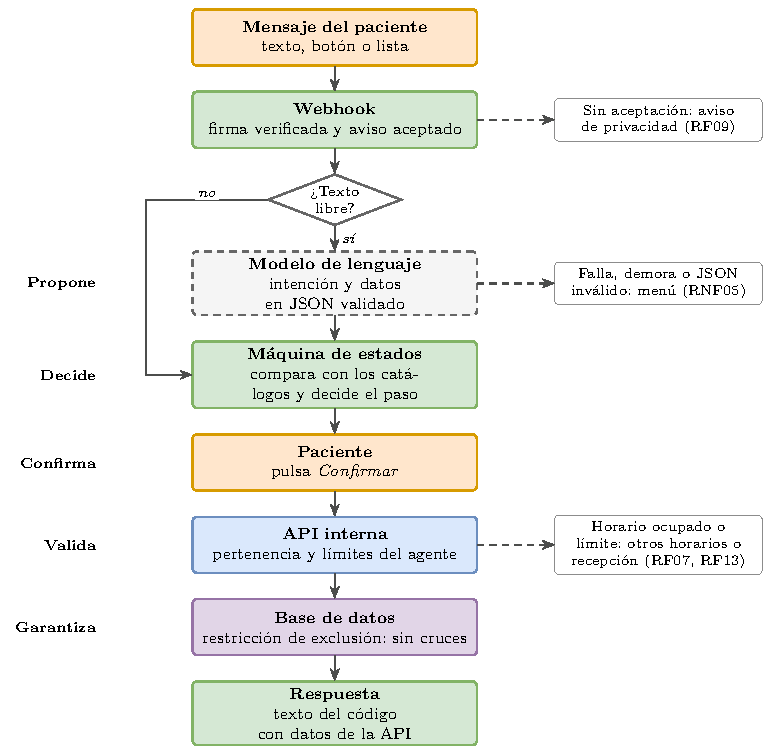
\includegraphics[width=0.85\linewidth]{img/Objetivo3/Ob3_Cadena_Decision.pdf}
\caption{Cadena de decisión de un mensaje en el agente híbrido}
\label{fig:ob3_cadena}
\end{figure}
